\section{The binomial option pricing model}
A relatively simple discrete time model for computing the price of an
American style option is the \emph{standard binomial model}
\cite{cox1979option}. 

The basic assumption is that the price of the underlying follows a
binomial process over equally spaced time steps. This makes it
possible to write out the possible future states of the
underlying. Moving a single time step forward, the binomial process
produces two possible future states of the underlying. The value of
the underlying can go either up or down with probabilities $q$ and $1
- q$ respectively. We denote the rate of up and down movement as $u$
and $d$ respectively. Thus, after one time period the current price
would have moved up to the new value $uS$ with probability $q$ or
otherwise down to the new value $dS$ with probability $1-q$.

We skip the discussion of how to compute the constants $q$, $u$ and
$d$ and refer to the original source of the model
\cite{cox1979option}. After several time steps the binomial process
will unfold into a lattice of possible futures states as shown in
Figure \ref{fig:binomial-tree}. In this example we have assumed that
$u$ and $d$ has been selected such that $u\cdot d = 1$, but that is
not necessarily the case.

\begin{figure}
  \centering
  \tikzstyle{nodestyle} = [text centered, minimum size=0.42cm, inner sep=0]

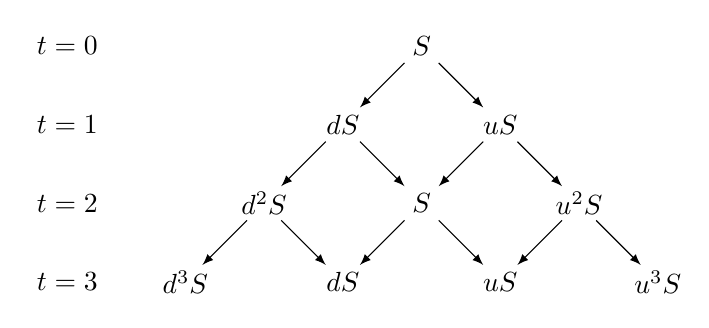
\begin{tikzpicture}
  \node at (0,0) [nodestyle] (S1) {$S$};

  \node at (-1, -1) [nodestyle] (dS) {$dS$};
  \node at ( 1, -1) [nodestyle] (uS) {$uS$};

  \node at ( 2, -2) [nodestyle] (u2S) {$u^2S$};
  \node at ( 0, -2) [nodestyle] (S2) {$S$};
  \node at (-2, -2) [nodestyle] (d2S) {$d^2S$};

  \node at ( 3, -3) [nodestyle] (u3S) {$u^3S$};
  \node at ( 1, -3) [nodestyle] (uS2) {$uS$};
  \node at (-1, -3) [nodestyle] (dS2) {$dS$};
  \node at (-3, -3) [nodestyle] (d3S) {$d^3S$};

  \node at (-4.5, 0) [] (t0) {$t=0$};
  \node at (-4.5, -1) [] (t0) {$t=1$};
  \node at (-4.5, -2) [] (t0) {$t=2$};
  \node at (-4.5, -3) [] (t0) {$t=3$};

  \path[-latex] 
     (S1) edge (uS)
     (S1) edge (dS)

     (uS) edge (S2)
     (dS) edge (S2)
     (uS) edge (u2S)
     (dS) edge (d2S)

     (u2S) edge (u3S)
     (u2S) edge (uS2)
     (S2)  edge (uS2)
     (S2)  edge (dS2)
     (d2S) edge (dS2)
     (d2S) edge (d3S);
\end{tikzpicture}

\vspace{2mm}

\caption{Lattice generated by the binomial process of a single
  underlying over three periods ($T=3$). The root
  node represents the current price of the underlying and the leafs
  represents possible values at expiration time.}
\label{fig:binomial-tree}
\end{figure}

The final row represents the possible values of the underlying at
expiration time, $T$, we can use the same procedure as for European
options (discussed above) to find the value of our option in each of
these cases. Thus, for each leaf node $i$, we compute the option value
as either $V_{i} = max(S_{i}-K, 0)$ for call options or $V_{i} =
max(K-S_{i},0)$ for put options, where $S_i$ is the price of the
underlying at node $i$, and $K$ being the strike price.

The algorithm now proceeds by estimating the price $V_i$ of the option
in the remaining lattice points. The price estimate at each lattice
point for time $t$ depends only on its two children at time
$t+1$. This is done recursively by:
$$V_{i} = e^{-r\Delta t} \cdot (q\cdot V_{\mathsf{left\textsf{-}child}(i)} + (1-q)\cdot V_{\mathsf{right\textsf{-}child}(i)})$$
where the probability $q$ is used to attain the expected value from
either of the two alternative futures, and $e^{r\Delta t}$ is the
guaranteed scale of increment over a single time period (following the
riskless rate $r$).

% \todo{Display the full binomial algorithm and parameters in a concise fact-box
% like format. Be sure to explain what $S(i,t)$ is.}

% In equations, this may be written as follows, where $x_{i,t}$ represents a
% lattice point.

% \begin{align*}
% v(x_{i,t}) &= h(f_{i,t}(v(x_{i,t+1})),g_{i,t}(v(x_{i+1,t+1}))) \\
% v(x_{i,T}) &= \max\{ 0, k - S(i,T) \} \tag{for a put-option}\\
% v(x_{i,T}) &= \max\{ 0, S(i,T) - k \} \tag{for a call-option}\\
% \end{align*}

% In our case the functions $f_{i,t},g_{i,t},h$ contain only simple constant-time
% arithmetic calculation.

\subsection{Implementation Techniques}

As seen above, the value of $V_i$ depends only on values associated
with time $t+1$. Therefore, for each $t$, the evaluation of $V_i$'s may
proceed in parallel.

Below, this is illustrated in pseudocode that uses only two arrays in
tandem to hold the intermediately produced values. It should also be
observed that it is not necessary to build the complete lattice, as we
are only interested in the values at expiration date.

\begin{algorithm}
% \begin{verbatim}
% binom:
%   -- A,B are assumed preallocated, and T is assumed odd.
%   t <- T
%   B <- parmap (\i -> max 0 (k-S(i,T))) [0..T]
%   while t > 0
%     A <- parmap (\i -> h(f_{i,t}(B[i]),g_{i,t}(B[i+1))) [0..t]
%     t <- t -1
%     B <- parmap (\i -> h(f_{i,t}(A[i]),g_{i,t}(A[i+1))) [0..t]
%     t <- t -1
%   return B
% \end{verbatim}

\begin{algorithmic}
\Function{Binom}{$\Delta t$, $T$, $u$, $d$, $q$, $S_0$, $K$, $r$}
  \State $A \gets \mathbf{alloc}\ T$
  \State $B \gets \mathbf{alloc}\ T$
  \State $B \gets \mathbf{parmap}$ $(\lambda i.\ d^{T-i}u^{i}S_0)$ $\{0..T\}$ \Comment Underlying value at expiration
  \State $B \gets \mathbf{parmap}$ $(\lambda S.\ \mathsf{max}\ 0\ (K-S))$ $B$ \Comment Perform exercise decision
  \State $t \gets T$
  \While{$t > 0$}
    \State $A \gets \mathbf{parmap}$ $(\lambda i.\ e^{-r\Delta t} \cdot (qB[i] + (1-q)B[i+1]))$ $\{0..t\}$
    \State $t \gets t-1$
    \State $B \gets \mathbf{parmap}$ $(\lambda i.\ e^{-r\Delta t} \cdot (qA[i] + (1-q)A[i+1]))$ $\{0..t\}$
    \State $t \gets t-1$
  \EndWhile
  \State \Return $B[0]$
\EndFunction
\end{algorithmic}
  
  \caption{Binomial algorithm}
  \label{alg:binomial-algorithm}
\end{algorithm}

\todo{cite blelloch} As defined by Blelloch (citation needed), the above code
may be reasonably assumed to have time complexities $Work(T^2/2)$ and
$Depth(T)$, and memory complexity $O(T)$.

While the above code is both short and simple in structure, the main motive for
pursuing parallelism is in gaining performance rather than expressivity.  To
explore further algorithm samples, we examine the binomial pricing algorithm
included in the CUDA SDK \cite{CUDAbinomial}.

\begin{verbatim}
lots of pseudocode.
\end{verbatim}

Notes: Duplication of computation, fixed amount of parallelism pr option being
priced, better scaling to pricing a larger number of options. Remark on the
poor scaling of the first algorithm.

%%% Local Variables:
%%% mode: latex
%%% TeX-master: "../master"
%%% End:
